\documentclass[a4paper]{article}
\usepackage{fontspec}
\usepackage{xeCJK}
\usepackage{amsmath}  % 必需的用于 \dfrac 的宏包
\usepackage[utf8]{inputenc}
\usepackage[chinese]{babel}
\usepackage{graphicx}
\usepackage{array}
\usepackage{fancyhdr}
\usepackage{lastpage} % 用于获取总页数的宏包
\usepackage{geometry} % 用于调整边距的宏包
\usepackage[datesep=/,style=ddmmyyyy]{datetime2} % 用于格式化日期的宏包
\usepackage{setspace} % 包含 setspace 宏包
\usepackage{enumitem}
\usepackage{amssymb} % 用于更多符号
\usepackage{indentfirst}
\usepackage{hyperref}
\usepackage{array}
\usepackage{booktabs}

\usepackage{titlesec} % 包含 titlesec 宏包
% 使用较小的字体重新定义章节标题格式
\titleformat{\section}
{\normalfont\large\bfseries}{\thesection}{1em}{}

% 定义页面和标题的边距
\geometry{
	left=20mm,
	right=20mm,
	top=40mm,
	bottom=30mm,
	headsep=20mm
}

\pagestyle{fancy}
\fancyhf{} % 清除默认的标题和页脚
\renewcommand{\headrulewidth}{0pt} % 删除标题中的线条
\renewcommand{\footrulewidth}{0.4pt} % 页脚上方的线条

\fancyhead[C]{ % 标题中的居中内容
	\begin{tabular}{|m{3.5cm}|m{9.0cm}|m{3.5cm}|}
		\hline
		\begin{minipage}[c][2.0cm][c]{3.5cm}
			\centering
			
\includegraphics[width=2.98cm,height=1.25cm]{logo.png}
		\end{minipage} & 
		\begin{minipage}[c][2.0cm][c]{9cm}
			\centering
			\hyphenpenalty=10000 % 避免断字
			\vspace*{\fill} % 文本前的灵活垂直间距
			\begin{spacing}{1.5} % 将行间距增加到 1.25
				{\large \textbf{用于减少电容器中的瞬态\textit{Inrush}电流的电感器}}
			\end{spacing}
			\vspace*{\fill} % 文本后的灵活垂直间距
		\end{minipage} & 
		\begin{minipage}[c][2.0cm][c]{3.5cm}
			\raggedleft
			发行日期: \DTMtoday \\
			页数: \thepage/\pageref{LastPage}
		\end{minipage} \\
		\hline
	\end{tabular}
}

% 页脚内容
\fancyfoot[L]{%
	\begin{tabular}[b]{@{}l@{}}
		\href{http://www.dax.energy}{www.dax.energy}
	\end{tabular}
}
\fancyfoot[C]{%
	\begin{tabular}[b]{@{}c@{}}
		\href{mailto:comercial@dax.energy}{comercial@dax.energy}
	\end{tabular}
}
\fancyfoot[R]{%
	\begin{tabular}[b]{@{}r@{}}
		+55 41 99940-3744 \\ 3626-2072
	\end{tabular}
}

\begin{document}
	\setstretch{1.25} % 将行间距设置为 1.25
	
	\section{背景}
	通过闭合断路器对电容器组进行激励(图 \ref{fig:picture1})将导致高的瞬态峰值电流(图 \ref{fig:picture2}),称为冲击电流。此瞬态峰值电流的幅值和频率是以下因素的函数:
	\begin{itemize}[label=\textendash]
		\item 施加的电压(闭合时电压波的点);
		\item 电路的等效电容;
		\item 电路中的电感(数量和位置);
		\item 闭合时电容器组中的电荷;
		\item 由于闭合电阻器或电路中其他电阻引起的任何阻尼。
	\end{itemize}
	
	\section{电容器组的输入数据}
	\begin{itemize}[label=\textendash]
		\item 无功功率  = {{potencia_reativa_do_banco}}
		\item 三相电压  = {{tensao_trifasica}}
		\item 单相电压  = {{tensao_monofasica}}
		\item 短路电流  = {{corrente_de_curto}}
	\end{itemize}
	
	\begin{center}
		% INSERT_TABLE_HERE
	\end{center}
	
	\section{初步考虑}
	
	瞬态\textit{Inrush}电流在独立电容器组应用中不是限制因素。然而,当电容器组被\textit{背靠背}切换时,即在一个组被激励时,而另一个组仍然连接到同一母线上,高幅值和自然频率的瞬态电流将流动在已激励的组和新激励的组之间。
	
	\begin{figure}[!hbp]
		\centering
		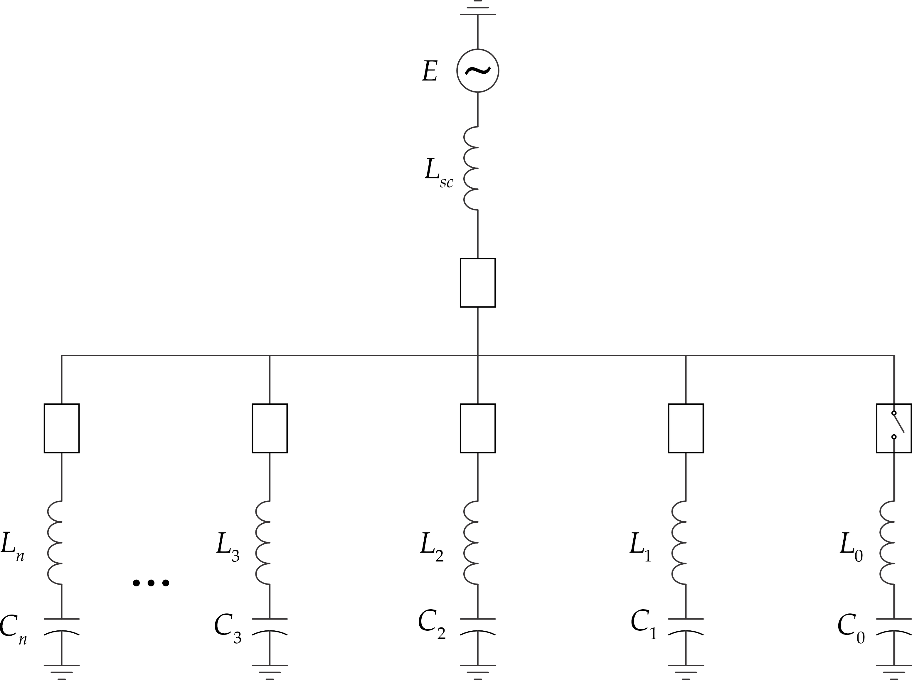
\includegraphics{Picture1.png}
		\caption{电容器组系统。}
		\label{fig:picture1}
	\end{figure}
	
	这种振荡电流仅受电容器组的阻抗以及已激励的组和切换组(组\#0)之间的电路的限制,通常在系统频率周期的一小部分内衰减至零。在\textit{背靠背}切换的情况下,电源提供的分量以较低的频率(60 Hz)存在,并且与\textit{Inrush}电流相比很小,可以忽略不计 \href{https://ieeexplore.ieee.org/document/7035261}{[ANSI/IEEE C37.012-1979]}。
	
	\section{结果}
	\begin{figure}[!hbp]
		\centering
		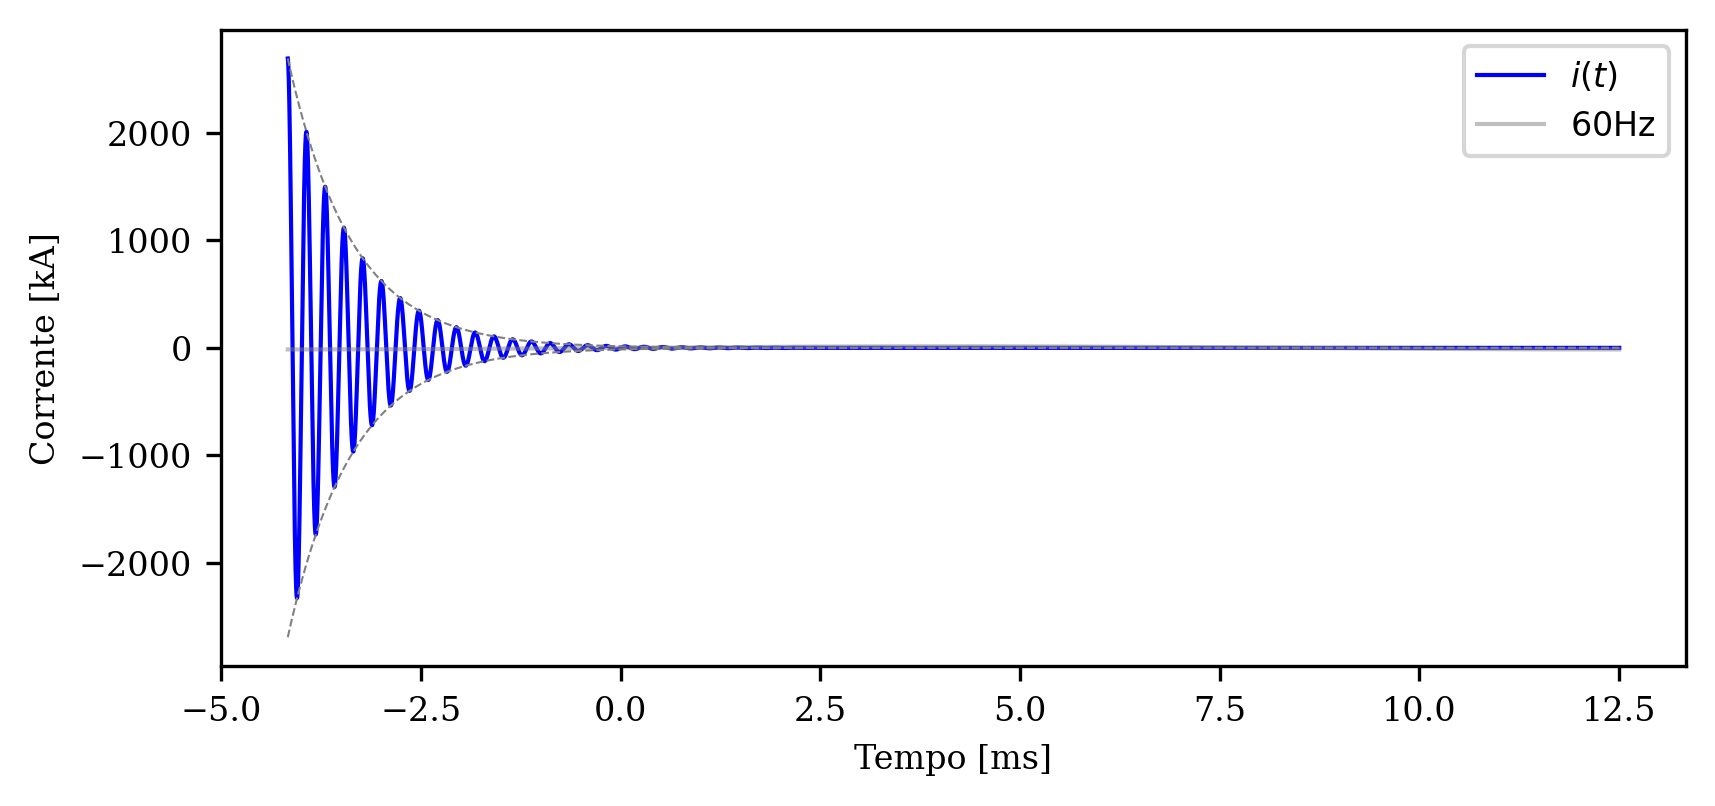
\includegraphics{Correntes.png}
		\caption{在一个基础频率周期内激励的电容器组中的瞬时电流。}
		\label{fig:picture2}
	\end{figure}
	
	使用选定的电感器($L_{reator} = {{indutancia_escolhida}} \, \mu \rm{H} $)获得的值为:
	\begin{itemize}[label=\textendash]
		\item 峰值电流: {{corrente_pico}};
		\item 振荡频率: {{frequencia_oscilacao}}Hz;
		\item 冲击电流 / 额定电流: {{inrush_inominal}}
	\end{itemize}
	
	\section{结论}
	{{conclusao1}}
	
	\section{参考文献}
	
	\noindent
	\begin{tabular}{p{0.2cm} p{15.8cm}}
		\href{https://ieeexplore.ieee.org/document/7035261}{[1]} &
		\begin{minipage}[t]{15.8cm}
			IEEE 应用指南关于对称电流基础上的 AC 高压断路器的电容电流切换,在 ANSI/IEEE C37.012-1979 中,vol.,no.,pp.1-54,1979 年 2 月 6 日,doi: 10.1109/IEEESTD.1979.7035261。
		\end{minipage} \\
		
		\href{https://ieeexplore.ieee.org/document/9574631}{[2]} &
		\begin{minipage}[t]{15.8cm}
			IEEE 批准的 AC 系统(1 kV 至 38 kV)电容器开关标准草案要求,在 IEEE PC37.66/D10 中,2021 年 10 月,vol.,no.,pp.1-35,2021 年 12 月 13 日。
		\end{minipage} \\
		
		
		\href{https://webstore.iec.ch/publication/62785}{[3]} &
		\begin{minipage}[t]{15.8cm}
			IEC 62271-100 高压开关设备和控制设备 - 第 100 部分:交流断路器
		\end{minipage} \\
		
		\href{https://ieeexplore.ieee.org/document/5318709}{[4]} &
		\begin{minipage}[t]{15.8cm}
			IEEE 标准关于对称电流基础上的 AC 高压断路器的额定值 - 电压超过 1000 V 的首选额定值和相关所需能力,在 IEEE Std C37.06-2009 中,vol.,no.,pp.1-56,2009 年 11 月 6 日,doi: 10.1109/IEEESTD.2009.5318709。
		\end{minipage} \\
		
		\href{https://cdn.standards.iteh.ai/samples/101972/4e7e06bd66d2443da668b8e0c6c60512/IEC-62271-100-2021.pdf}{[5]} &
		\begin{minipage}[t]{15.8cm}
			IEC 62271-100 高压开关设备和控制设备 – 第 100 部分:交流断路器。
		\end{minipage} \\
		
		\href{https://www.normas.com.br/autorizar/visualizacao-nbr/313/identificar/visitante}{[6]} &
		\begin{minipage}[t]{15.8cm}
			NBR 5282 适用于额定电压超过 1000 V 的系统的并联电力电容器。
		\end{minipage} \\
	\end{tabular}
	
	% 签名空间
	\noindent % 防止缩进
	\begin{minipage}[t]{0.5\textwidth} % 开始签名的第一列
		\centering % 将文本对齐到中心
		\vspace{5cm} % 为签名预留空间
		\rule{6cm}{0.4pt}\\ % 签名线
		\textbf{Angelo A. Hafner}\\ % 名称
		电气工程师\\ % 职称
		CONFEA: 2.500.821.919\\ % 注册号
		CREA/SC: 045.776-5\\ % 另一个注册号
		aah@dax.energy % 电子邮件
	\end{minipage}%
	\hfill % 列间空隙
	\begin{minipage}[t]{0.5\textwidth} % 开始签名的第二列
		\centering % 将文本对齐到中心
		\vspace{5cm} % 为签名预留空间
		\rule{6cm}{0.4pt}\\ % 签名线
		\textbf{Tiago Machado}\\ % 名称
		业务经理\\ % 职称
		手机: +55 41 99940-3744\\ % 联系方式
		tm@dax.energy % 电子邮件
	\end{minipage}
	
\end{document}
